\documentclass{beamer}

\usepackage{hyperref}
\usepackage{graphicx}
\graphicspath{ {images/} }
\usepackage{tabularx}

\usetheme{Madrid}
\usecolortheme{default}
\setbeamertemplate{navigation symbols}{}

\begin{document}

\title{Gamification of Clinical Practice Guidelines}
\author{Ben-Richard Ebbesvik}
\institute{Western Norway University of Applied Sciences \newline University of Bergen}
\date{3rd of April 2019}
\subject{Master thesis}
\frame{\titlepage}


\begin{frame}{Introduction}
Clinical Practice Guidelines are documents that contain recommendations to assist clinicians providing optimized health care, based on latest evidence. 

Advantages:
\begin{itemize}
	\item Clinicians don't have to search through and review an overwhelming amount of research articles to keep up to date with the latest best evidence .
	\item Improved quality of health care (benefits and harm).
	\item Reduce practice variability.
	\item Reduce cost of health care.
\end{itemize}	
%\begin{block}{Definition}	
%	 "Clinical Practice Guidelines are statements that include recommendations intended to optimize patient care that are informed by a systematic review of evidence and an assessment of the cost, benefits and harms of alternative care options." (The Institute of Medicine 2011)
%\end{block}
\end{frame}

\begin{frame}{Introduction}
Despite the advantages, Clinical Practice Guidelines have had an limited effect on changing clinicians practice methods.
\begin{itemize}
	\item Lack of awareness.
	\item Lack of familiarity.
	\item  Lack of self-efficacy.
	\item Not easy to use, inconvenient, cumbersome
	\item +++
\end{itemize}
Example: Guidelines for the Diagnosis and Management of Asthma consists of 440 pages.
%Our contribution: a game.
\end{frame}

\begin{frame}{Possible asthma in paediatrics - Norway}
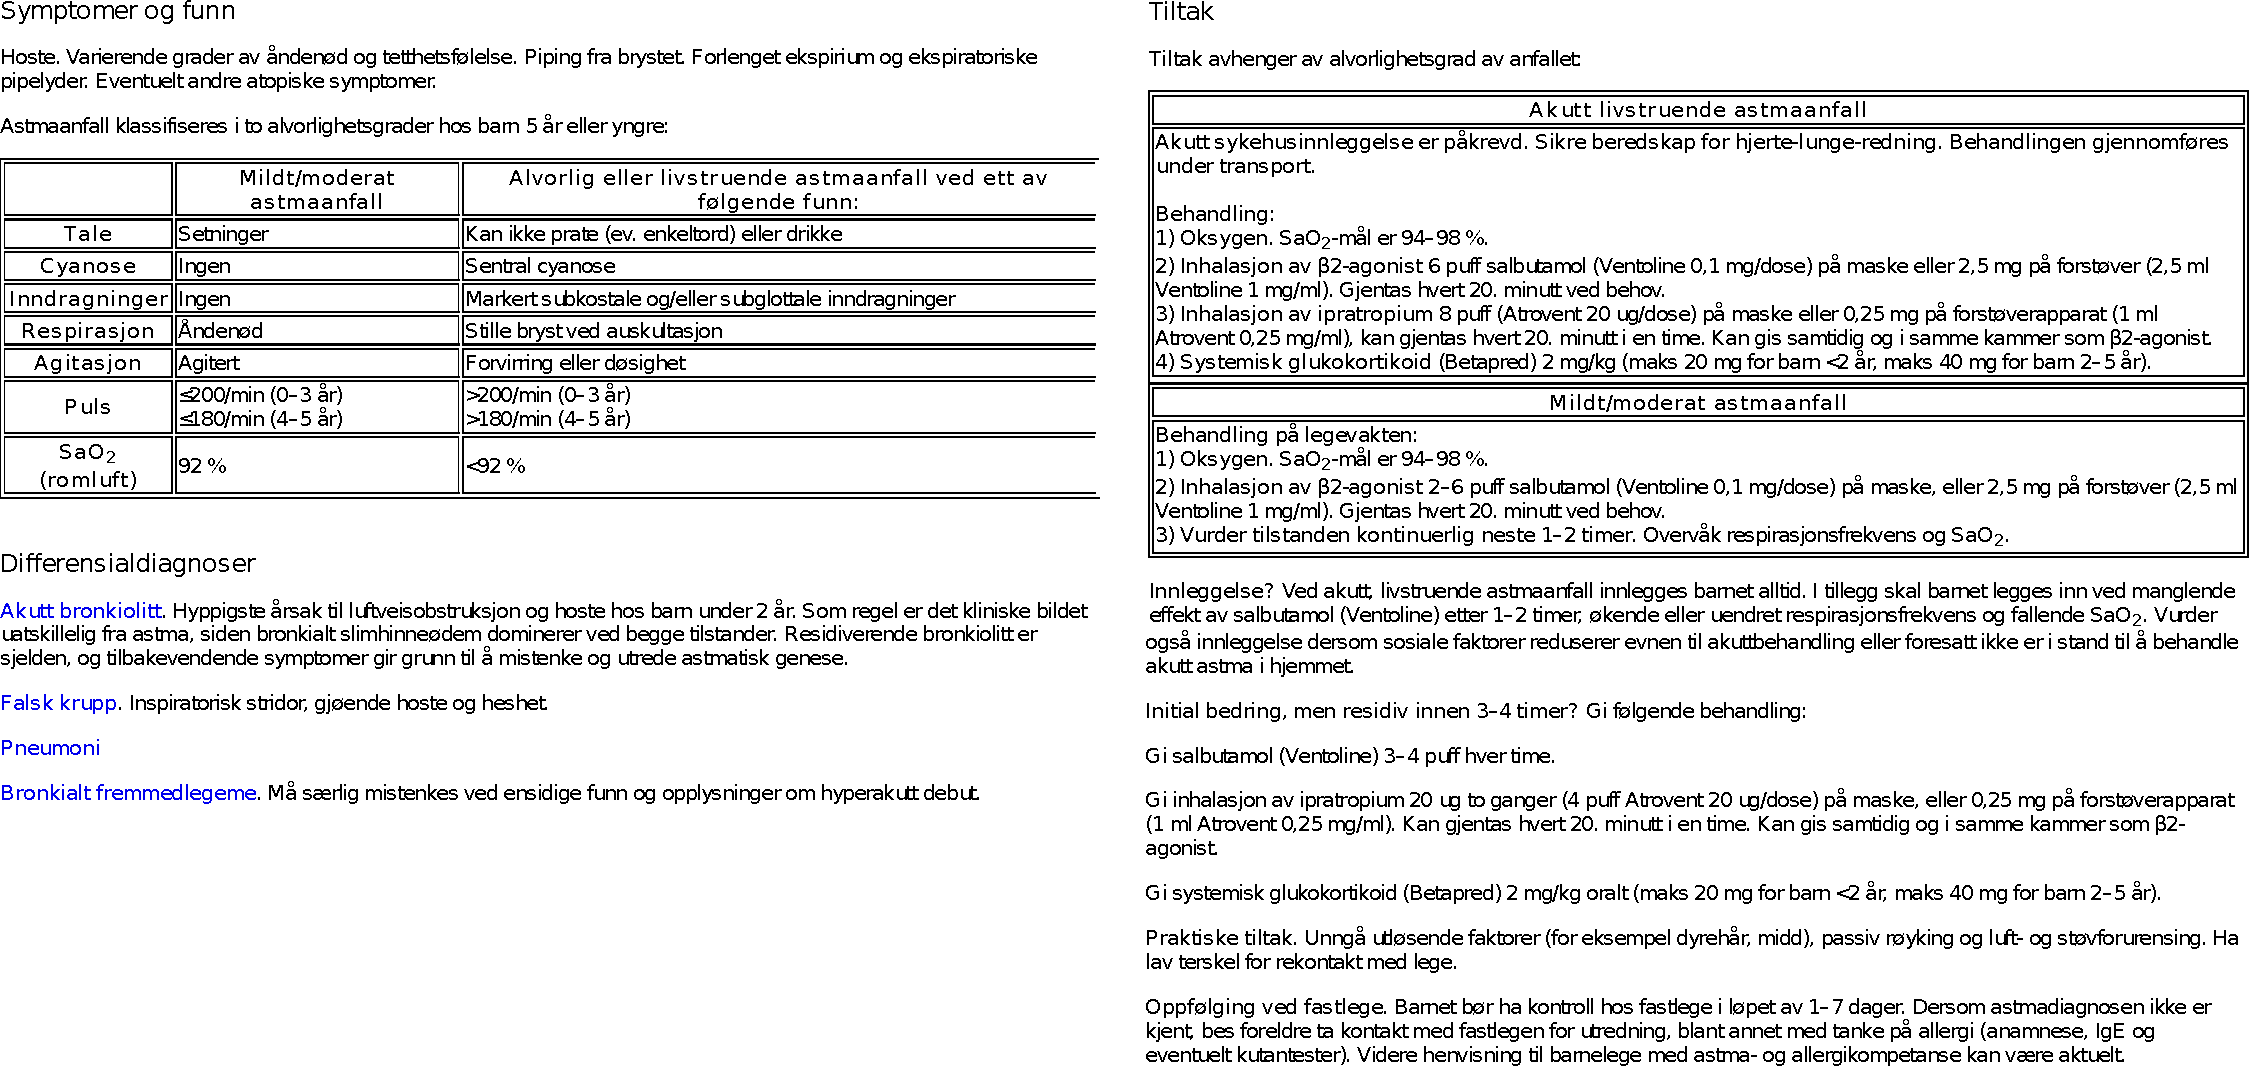
\includegraphics[scale=0.32]{NorwayCPG}
\end{frame}


\begin{frame}{Research questions}
\begin{itemize}
		%\item Based on clinical guidelines, can we make a reusable data structure representing respiratory diseases for use in serious games?
		\item Based on clinical guidelines, can we make a data structure which is easy to implement in the system, as well as adaptable? 
	
			\item How to use such a model for generating and testing case based multiple choice questions and answer elements?
			%\item Can we use the data model to structure the learning content such that it is adapted to the current knowledge of the individual learner?
			
	
	\item How can we model the work-flow of a clinical encounter, a patient at a given point in the clinical encounter, and a student at the current point in his learning process. How to represent these?	
\end{itemize}
\end{frame}


\begin{frame}{Approach}
Design science
\begin{itemize}
	\item Problem: CPGs have proven to have a great potential, but are not used enough.
	\item Design an artefact that will contribute to more use of CPGs.
	\item Evaluation of the artefact will give us more knowledge around the domain and challenges. The research will come from the design. Improve and adjust the artefact accordingly. 
	\item Iterate and increment.
	\item Get more knowledge for medicine- and computer science. Scientific contribution.
\end{itemize}
\end{frame}

\begin{frame}{Gamification of Clinical Practice Guidelines}
\begin{itemize}
	\item A game in a quiz format for learning the content of CPGs.
	\item Multiple-choice and multiple-try with feedback.
	\item Adaptive to the individual learner.
	\item Intended for medical students and clinicians.
\end{itemize}
\end{frame}

\begin{frame}{Possible asthma in paediatrics - Kenya}
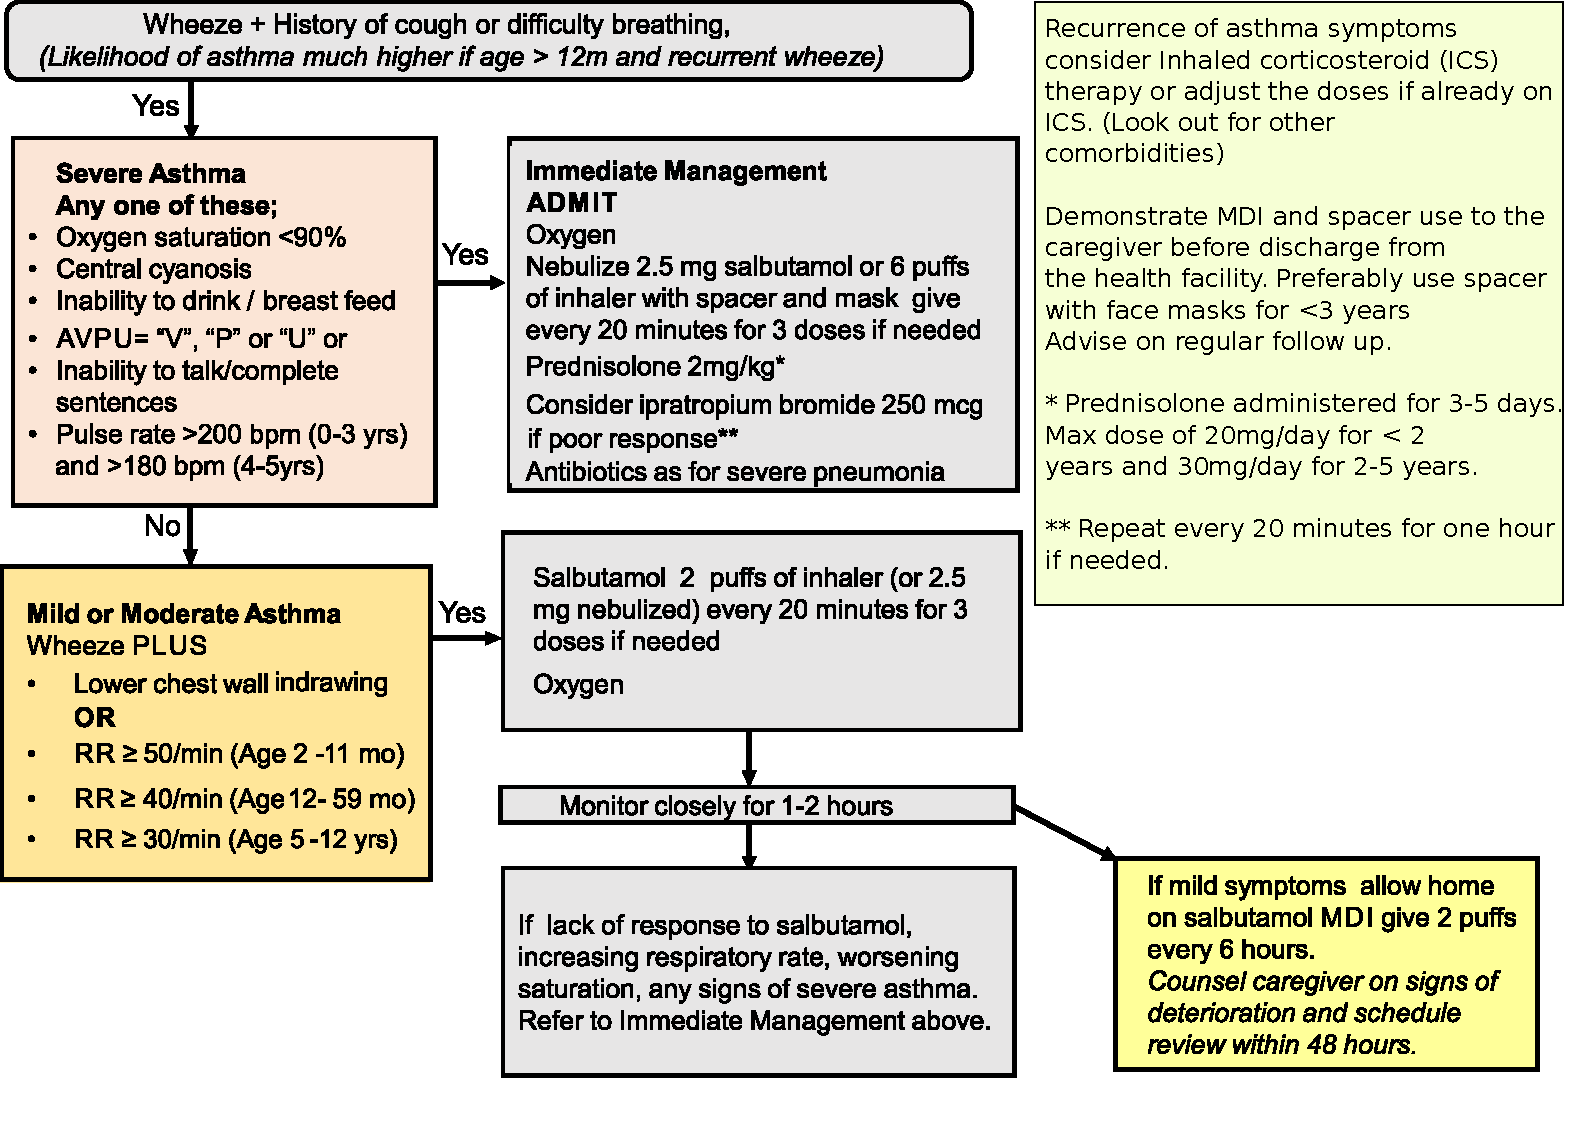
\includegraphics[scale=0.45]{KenyaCPG}
\end{frame}

\begin{frame}{Workflow graph}
The workflow graph is a model of the different steps through a clinical encounter.
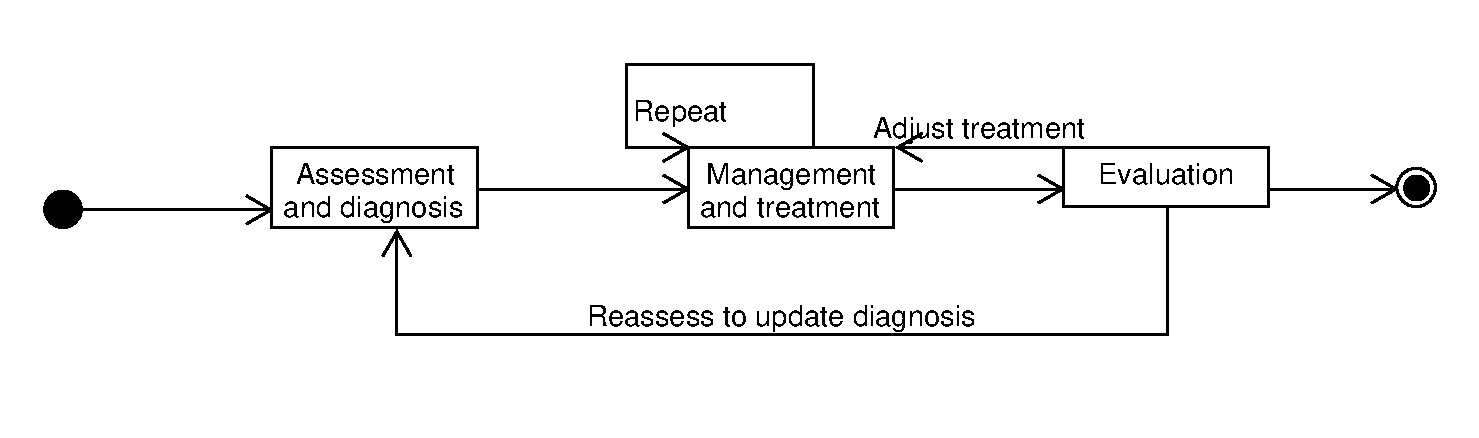
\includegraphics[scale=0.44]{WorkflowGraph}
\end{frame}

\begin{frame}{Excerpt of the entity graph}
The entity graph is a model of a patient at a given time.
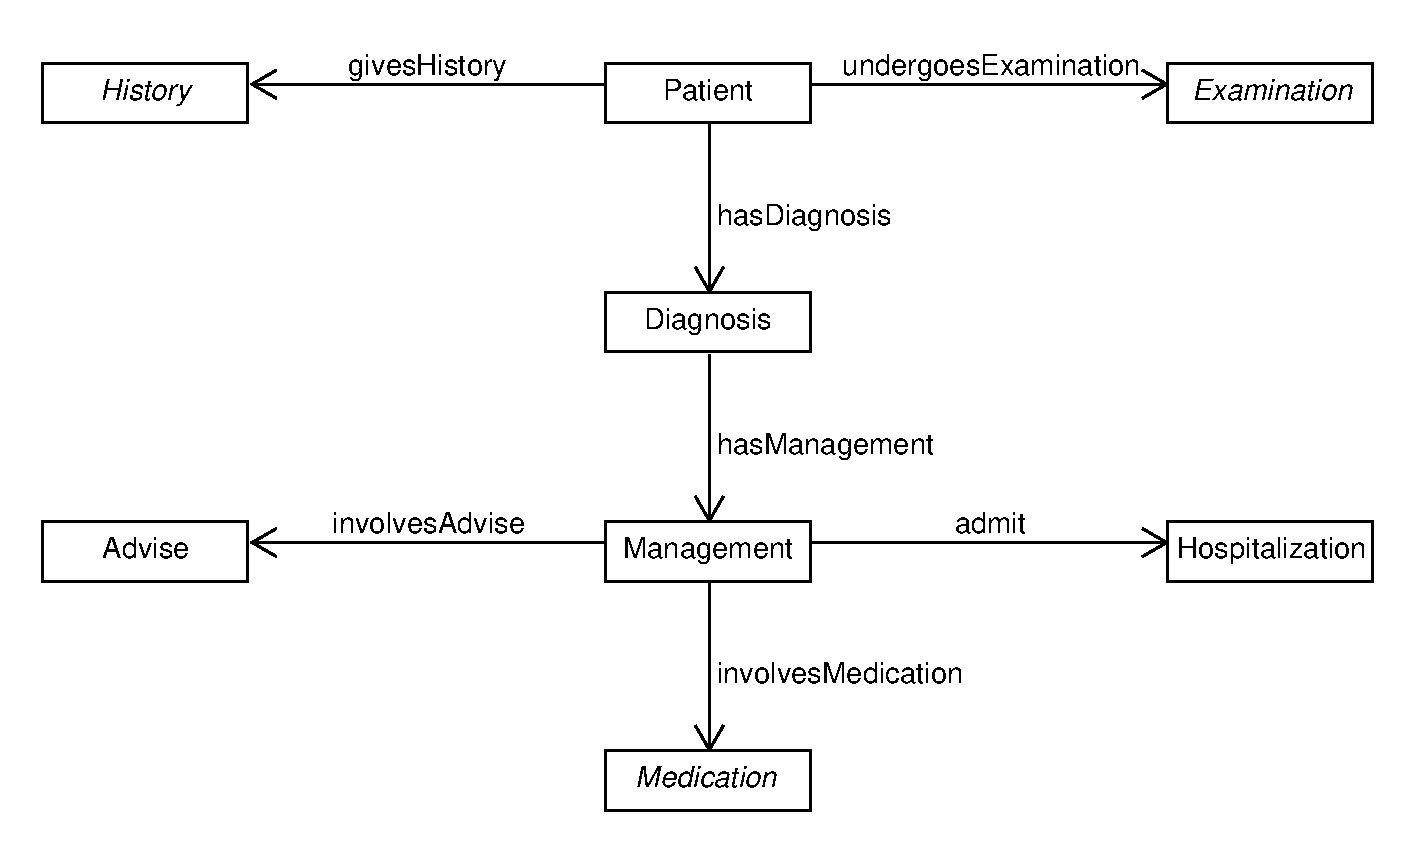
\includegraphics[scale=0.45]{SimpleEntityGraph}
\end{frame}


\begin{frame}[fragile]
\frametitle{Making scenarios, answer keys, distractions}
An instance of the entity model.
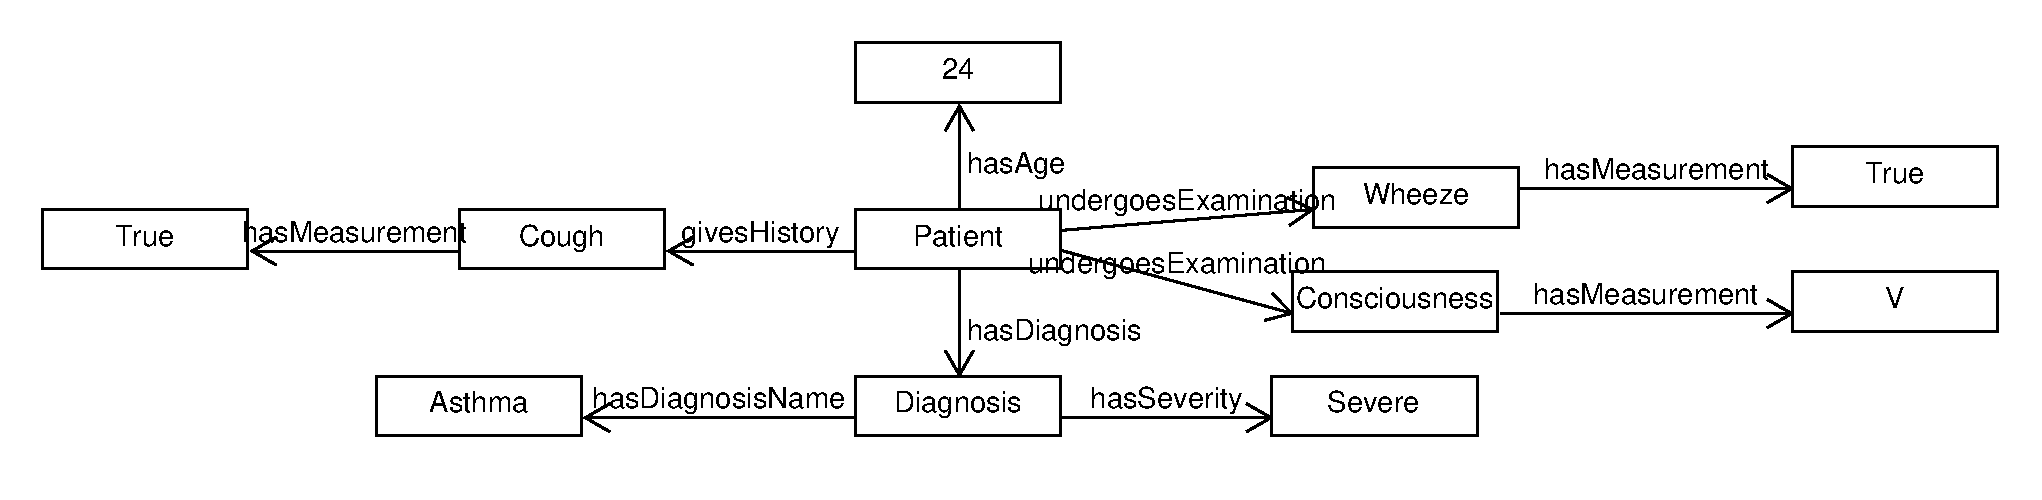
\includegraphics[scale=0.35]{EntityInstanceGraph}
\begin{semiverbatim}
A <\%Patient.hasAge.Age\%> old has arrived at the 
emergency clinic.  
She <\%Patient.givesHistory.Cough\%> 
<\%Patient.undergoesExamination.Wheeze\%>
<\%Patient.undergoesExamination.Consciousness\%>
\end{semiverbatim}
\end{frame}

\begin{frame}[fragile]
\frametitle{Making scenarios}
Adding presentation vertices to the instance.
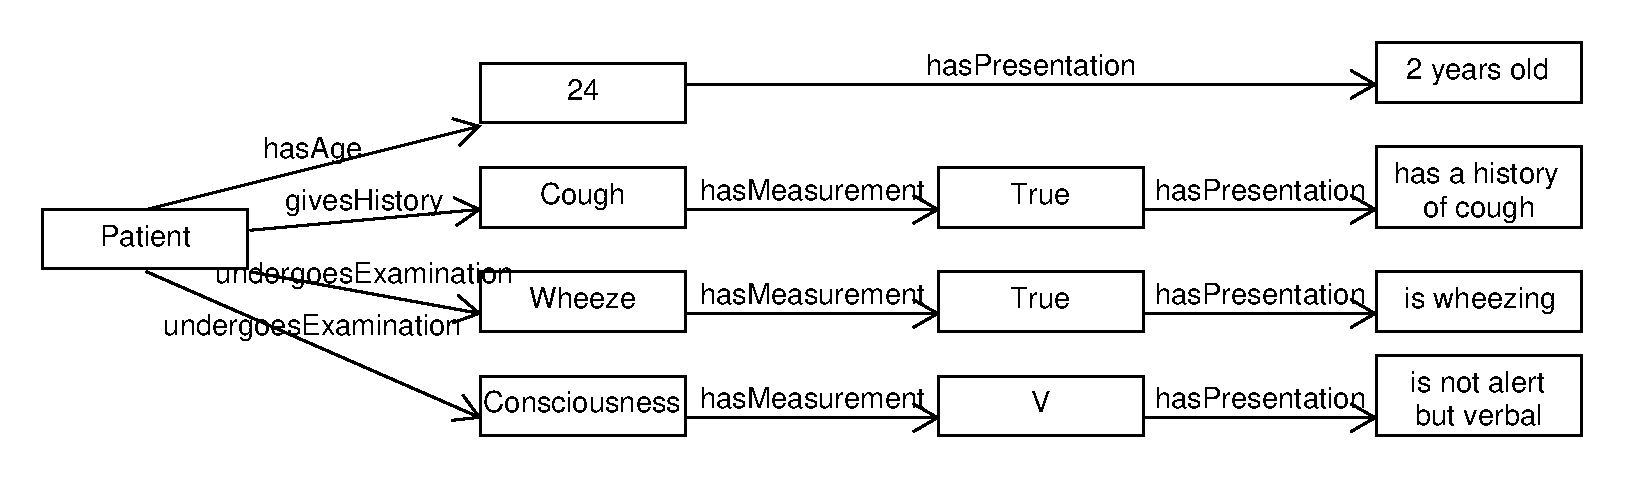
\includegraphics[scale=0.45]{PresentationEntityGraph}
\begin{semiverbatim}
	A 2 year old has arrived at the 
	emergency clinic.  
	She has a history of cough, 
	is wheezing
	and is not alert but verbal.
\end{semiverbatim}
\end{frame}

\begin{frame}{Dynamic Content Management}
\begin{itemize}
	\item Adaptive learning. Students will solve problems which are suited to their level of knowledge.
	\item Flexibility in the learning process. As long as the students follow the knowledge dependencies, they can go through the learning material in many different ways.
\end{itemize}
\end{frame}


\begin{frame}{Dynamic Content Management}
\begin{itemize}
	\item Split the learning content into atomic units of knowledge.
	\item Build up courses (quizzes) by selecting and organizing the knowledge units.
	\item Identify dependencies between the knowledge units.
\end{itemize}
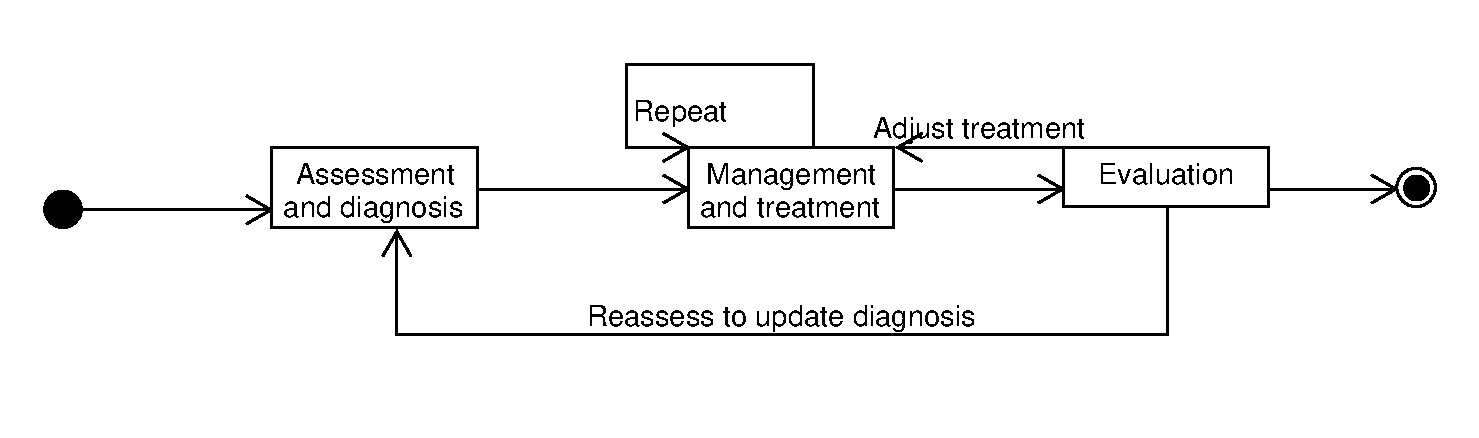
\includegraphics[scale=0.44]{WorkflowGraph}
%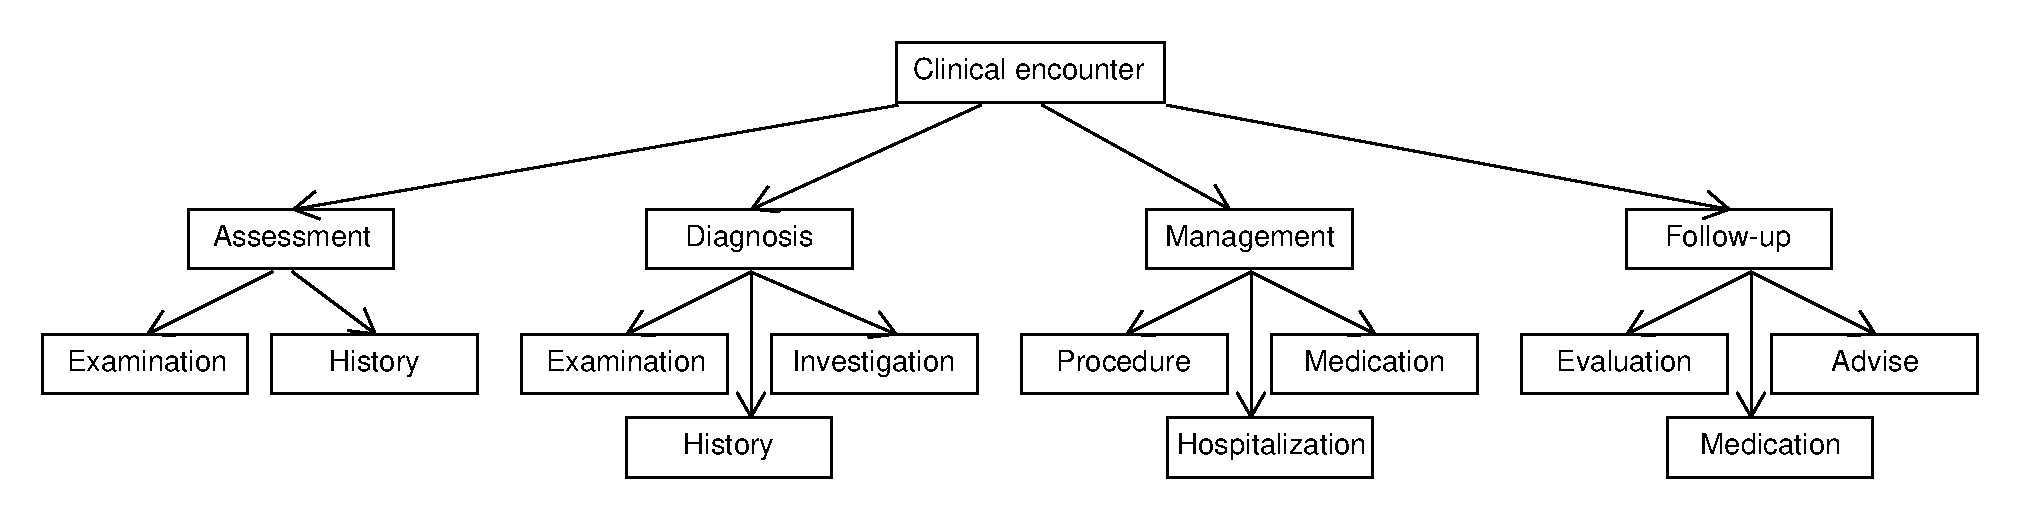
\includegraphics[scale=0.36]{KnowledgeMap}
\end{frame}

\begin{frame}{Dynamic Content Management}
Knowledge Map shows the dependencies in the learning process. 
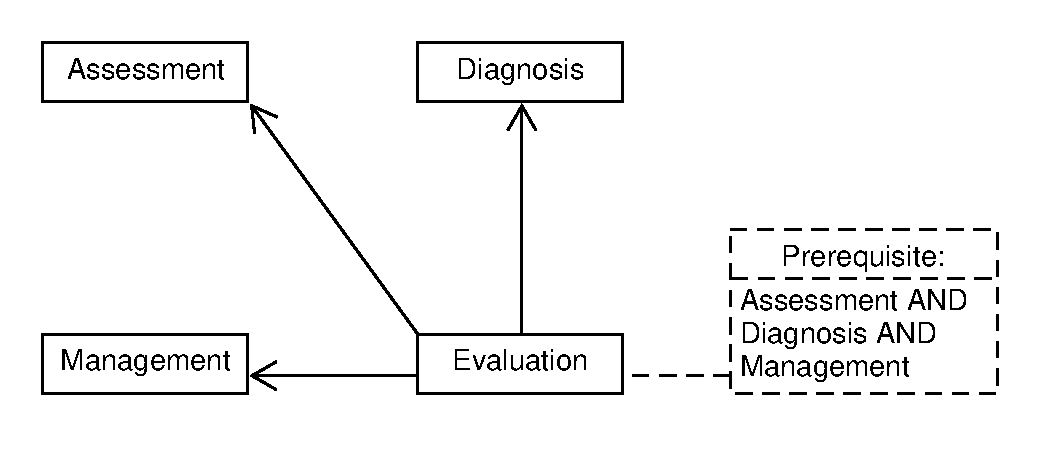
\includegraphics[scale=0.5]{Knowledge}
\end{frame}

\begin{frame}{Dynamic Content Management}
\begin{table}[h!]
\begin{tabular}{|m{2em}|m{6em}|m{6em}|m{6em}|m{6em}|}
	\hline
	 Level & Assessment & Diagnosis & Management & Follow-up \\
	\hline
	1  & Factual & Factual & Factual & - \\
	2 & Scenario & Scenario & Scenario & Scenario \\
	3 & Detailed scenario  & Detailed scenario & Detailed scenario & Detailed scenario \\
	\hline
\end{tabular}
\end{table}
\begin{itemize}
	\item Learning map shows all paths through the learning material.
	\item Student map shows one student's path in the learning map.
\end{itemize}
\end{frame}


\begin{frame}{Demonstration}
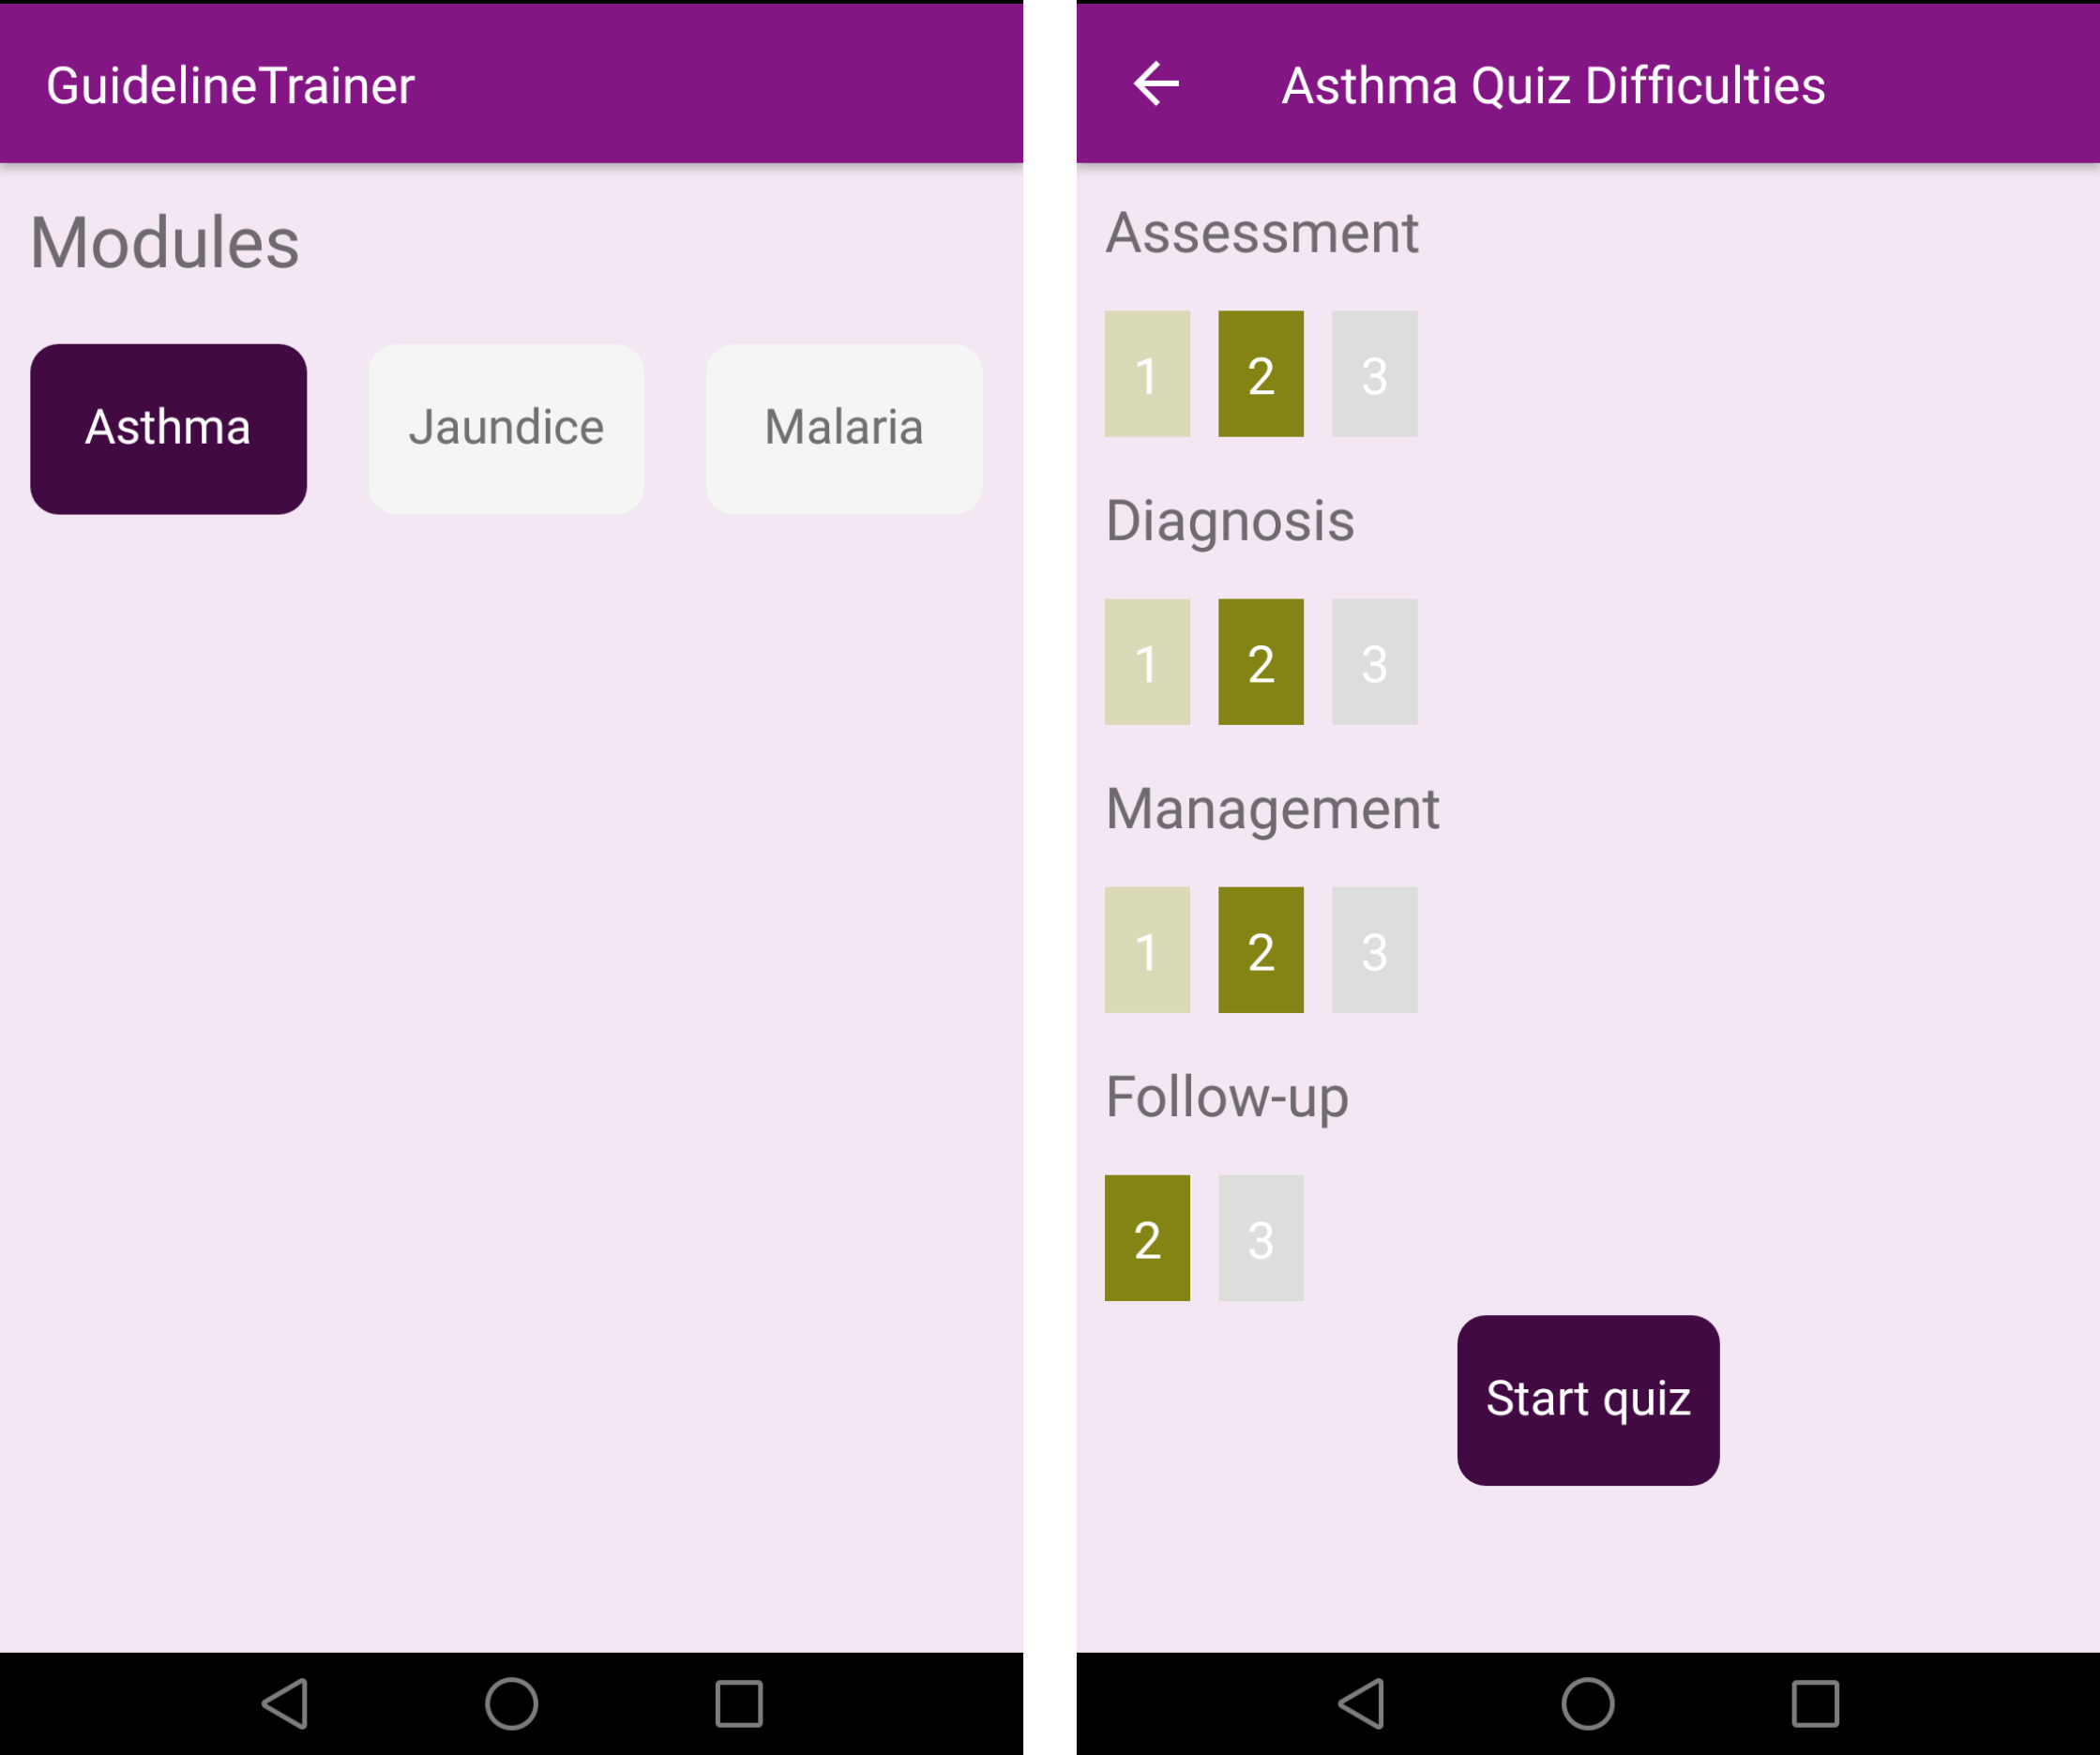
\includegraphics[scale=0.16]{Montage1}
\end{frame}
\begin{frame}{Demonstration}
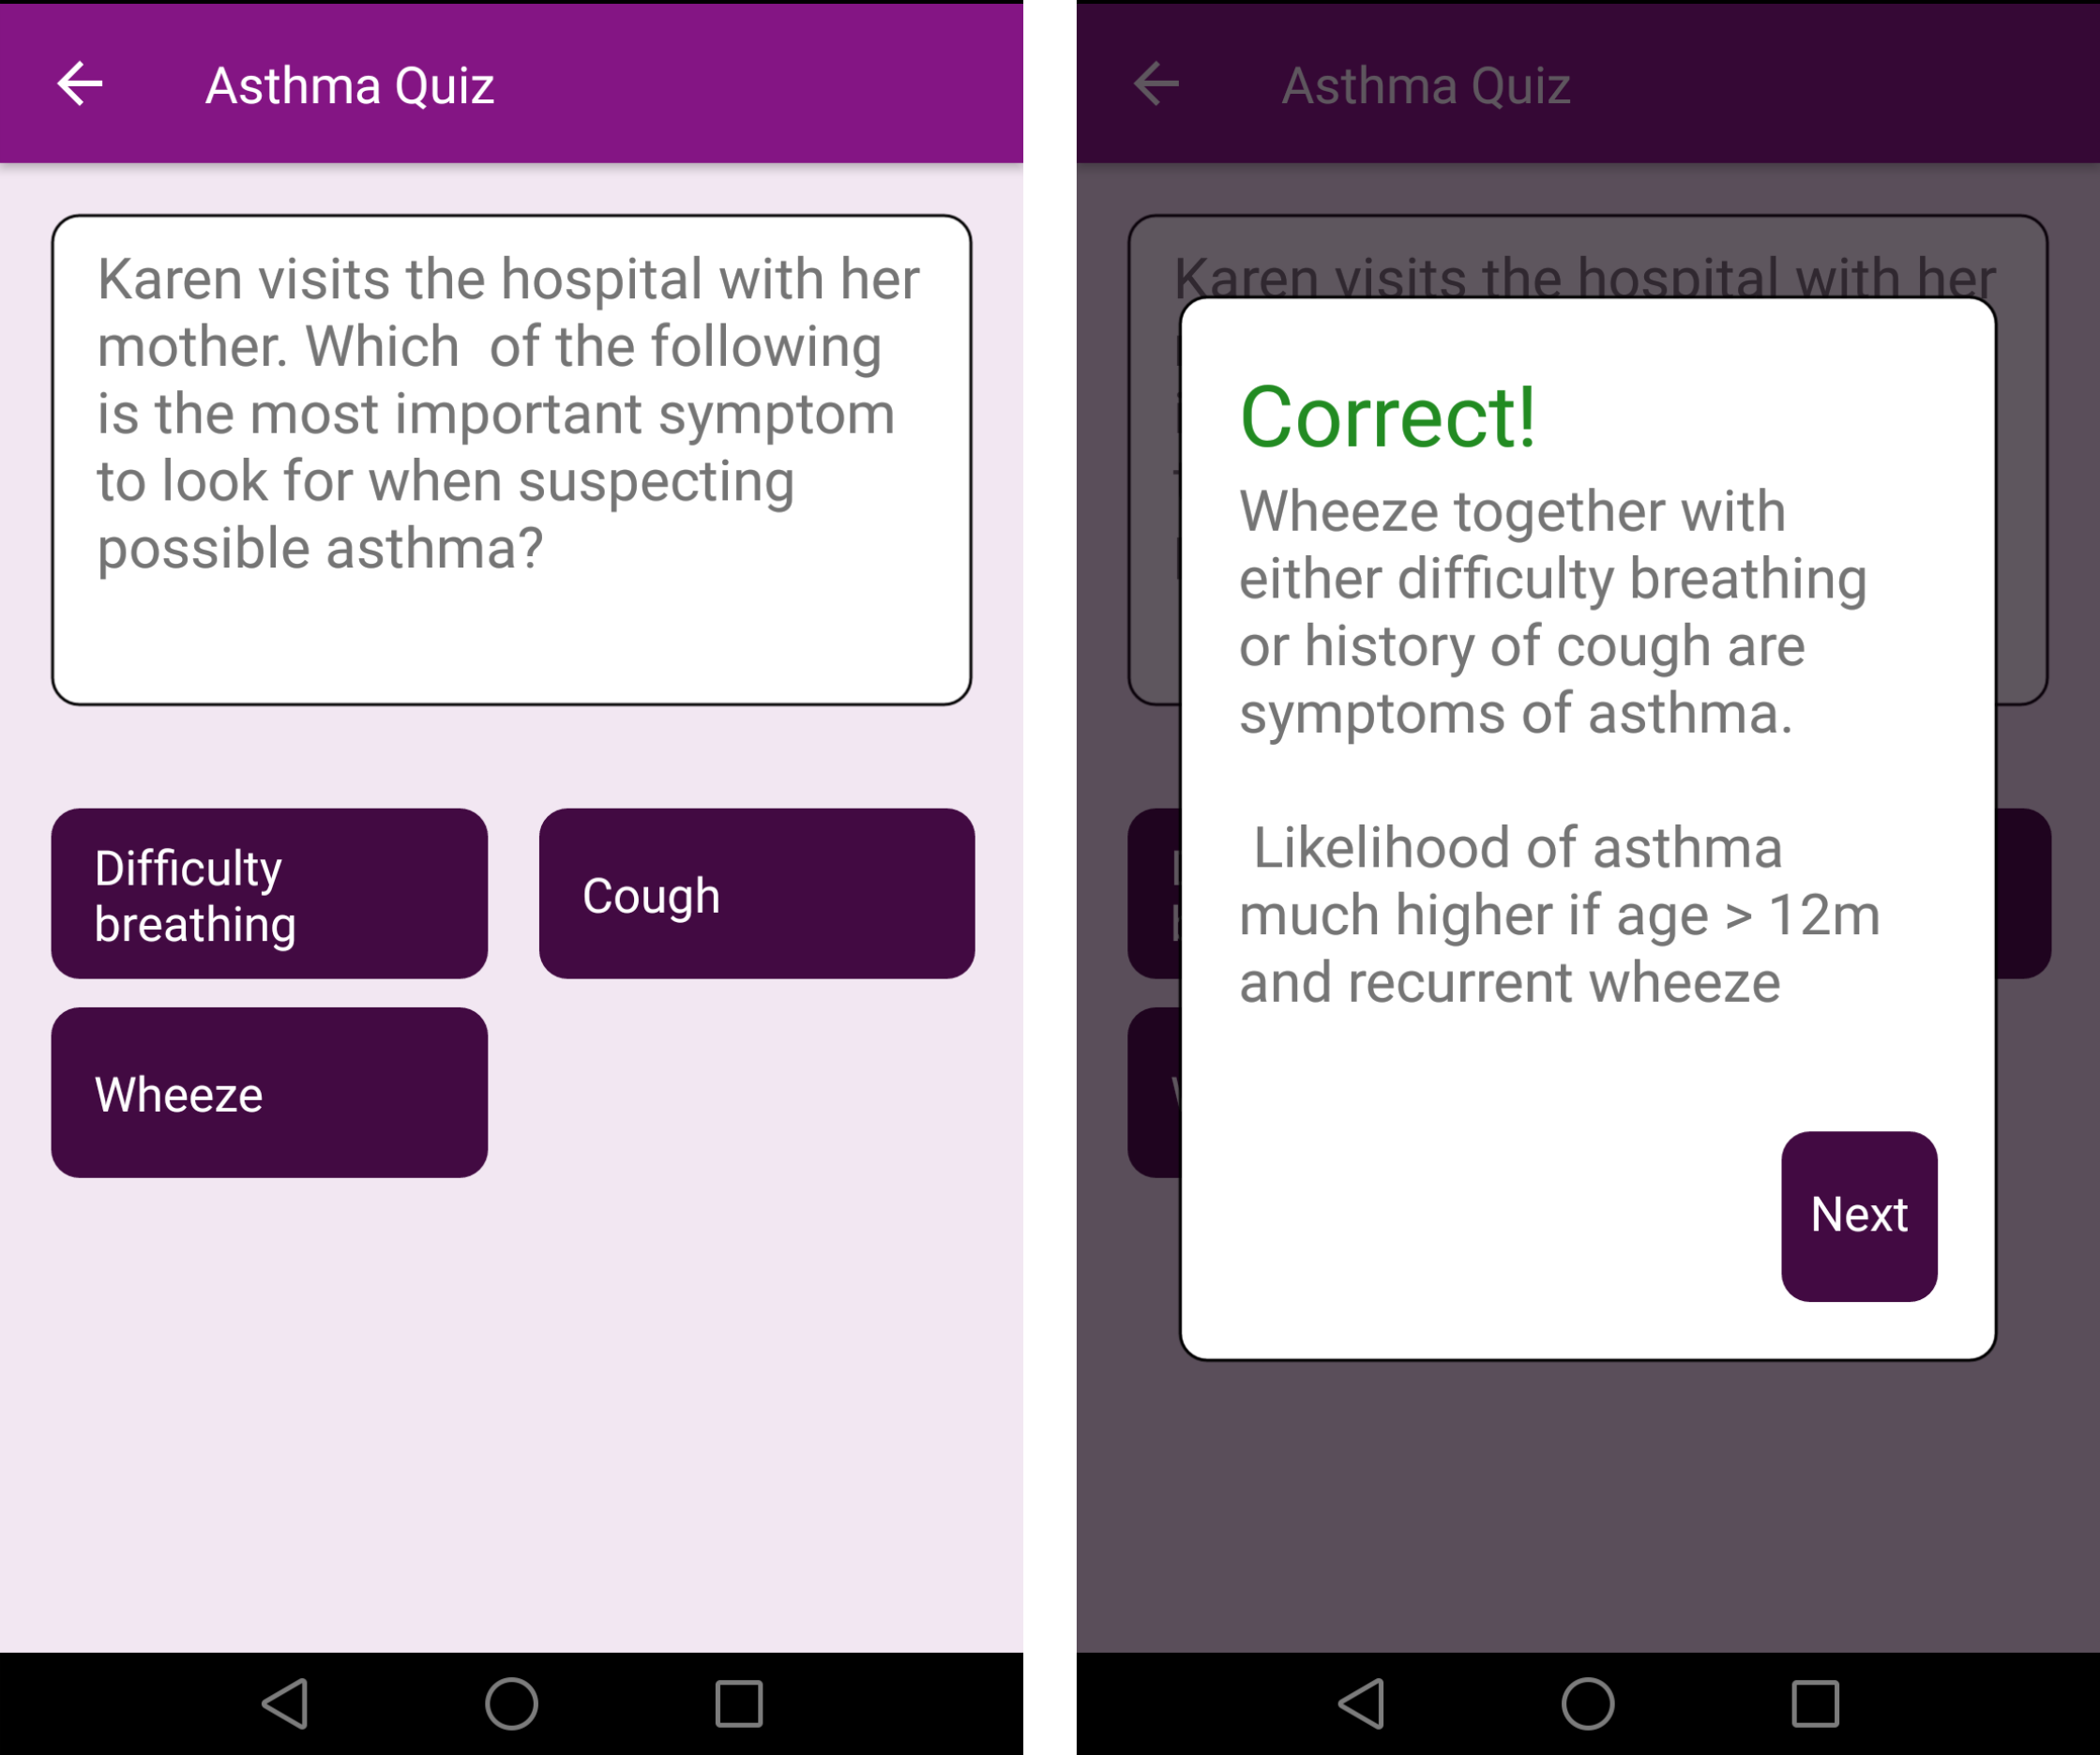
\includegraphics[scale=0.16]{Montage2}
\end{frame}
\begin{frame}{Demonstration}
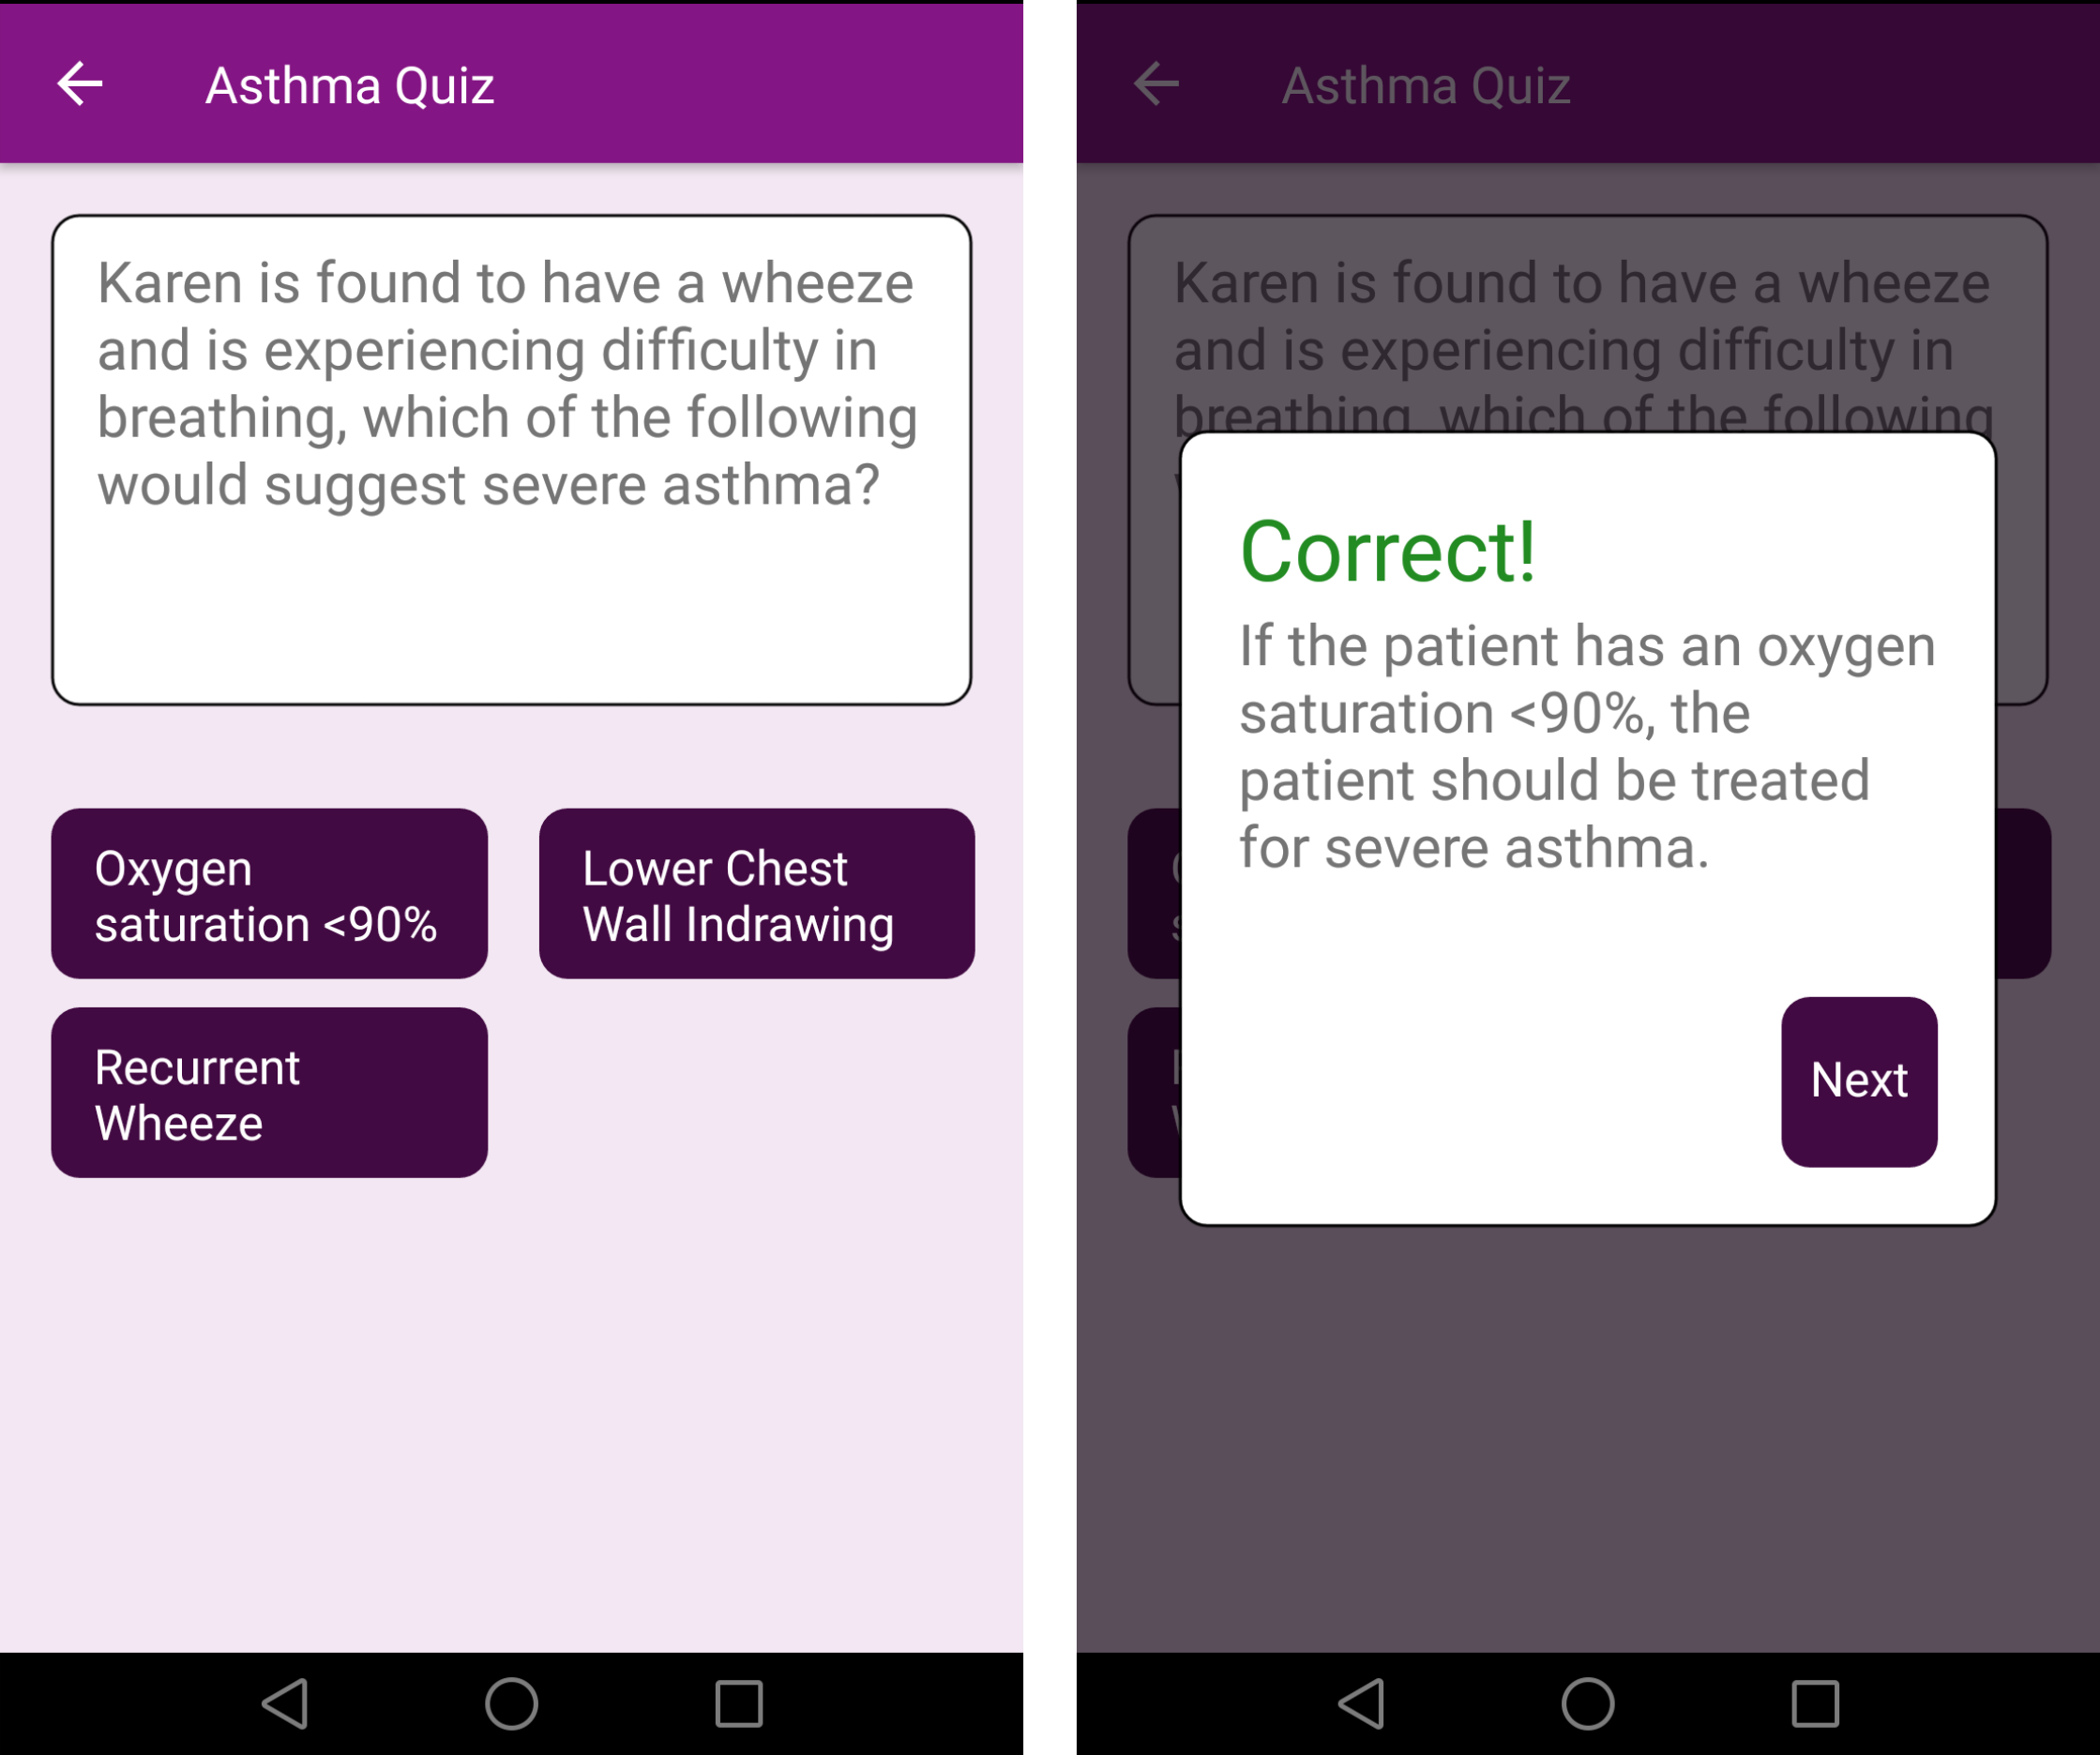
\includegraphics[scale=0.16]{Montage3}
\end{frame}
\begin{frame}{Demonstration}
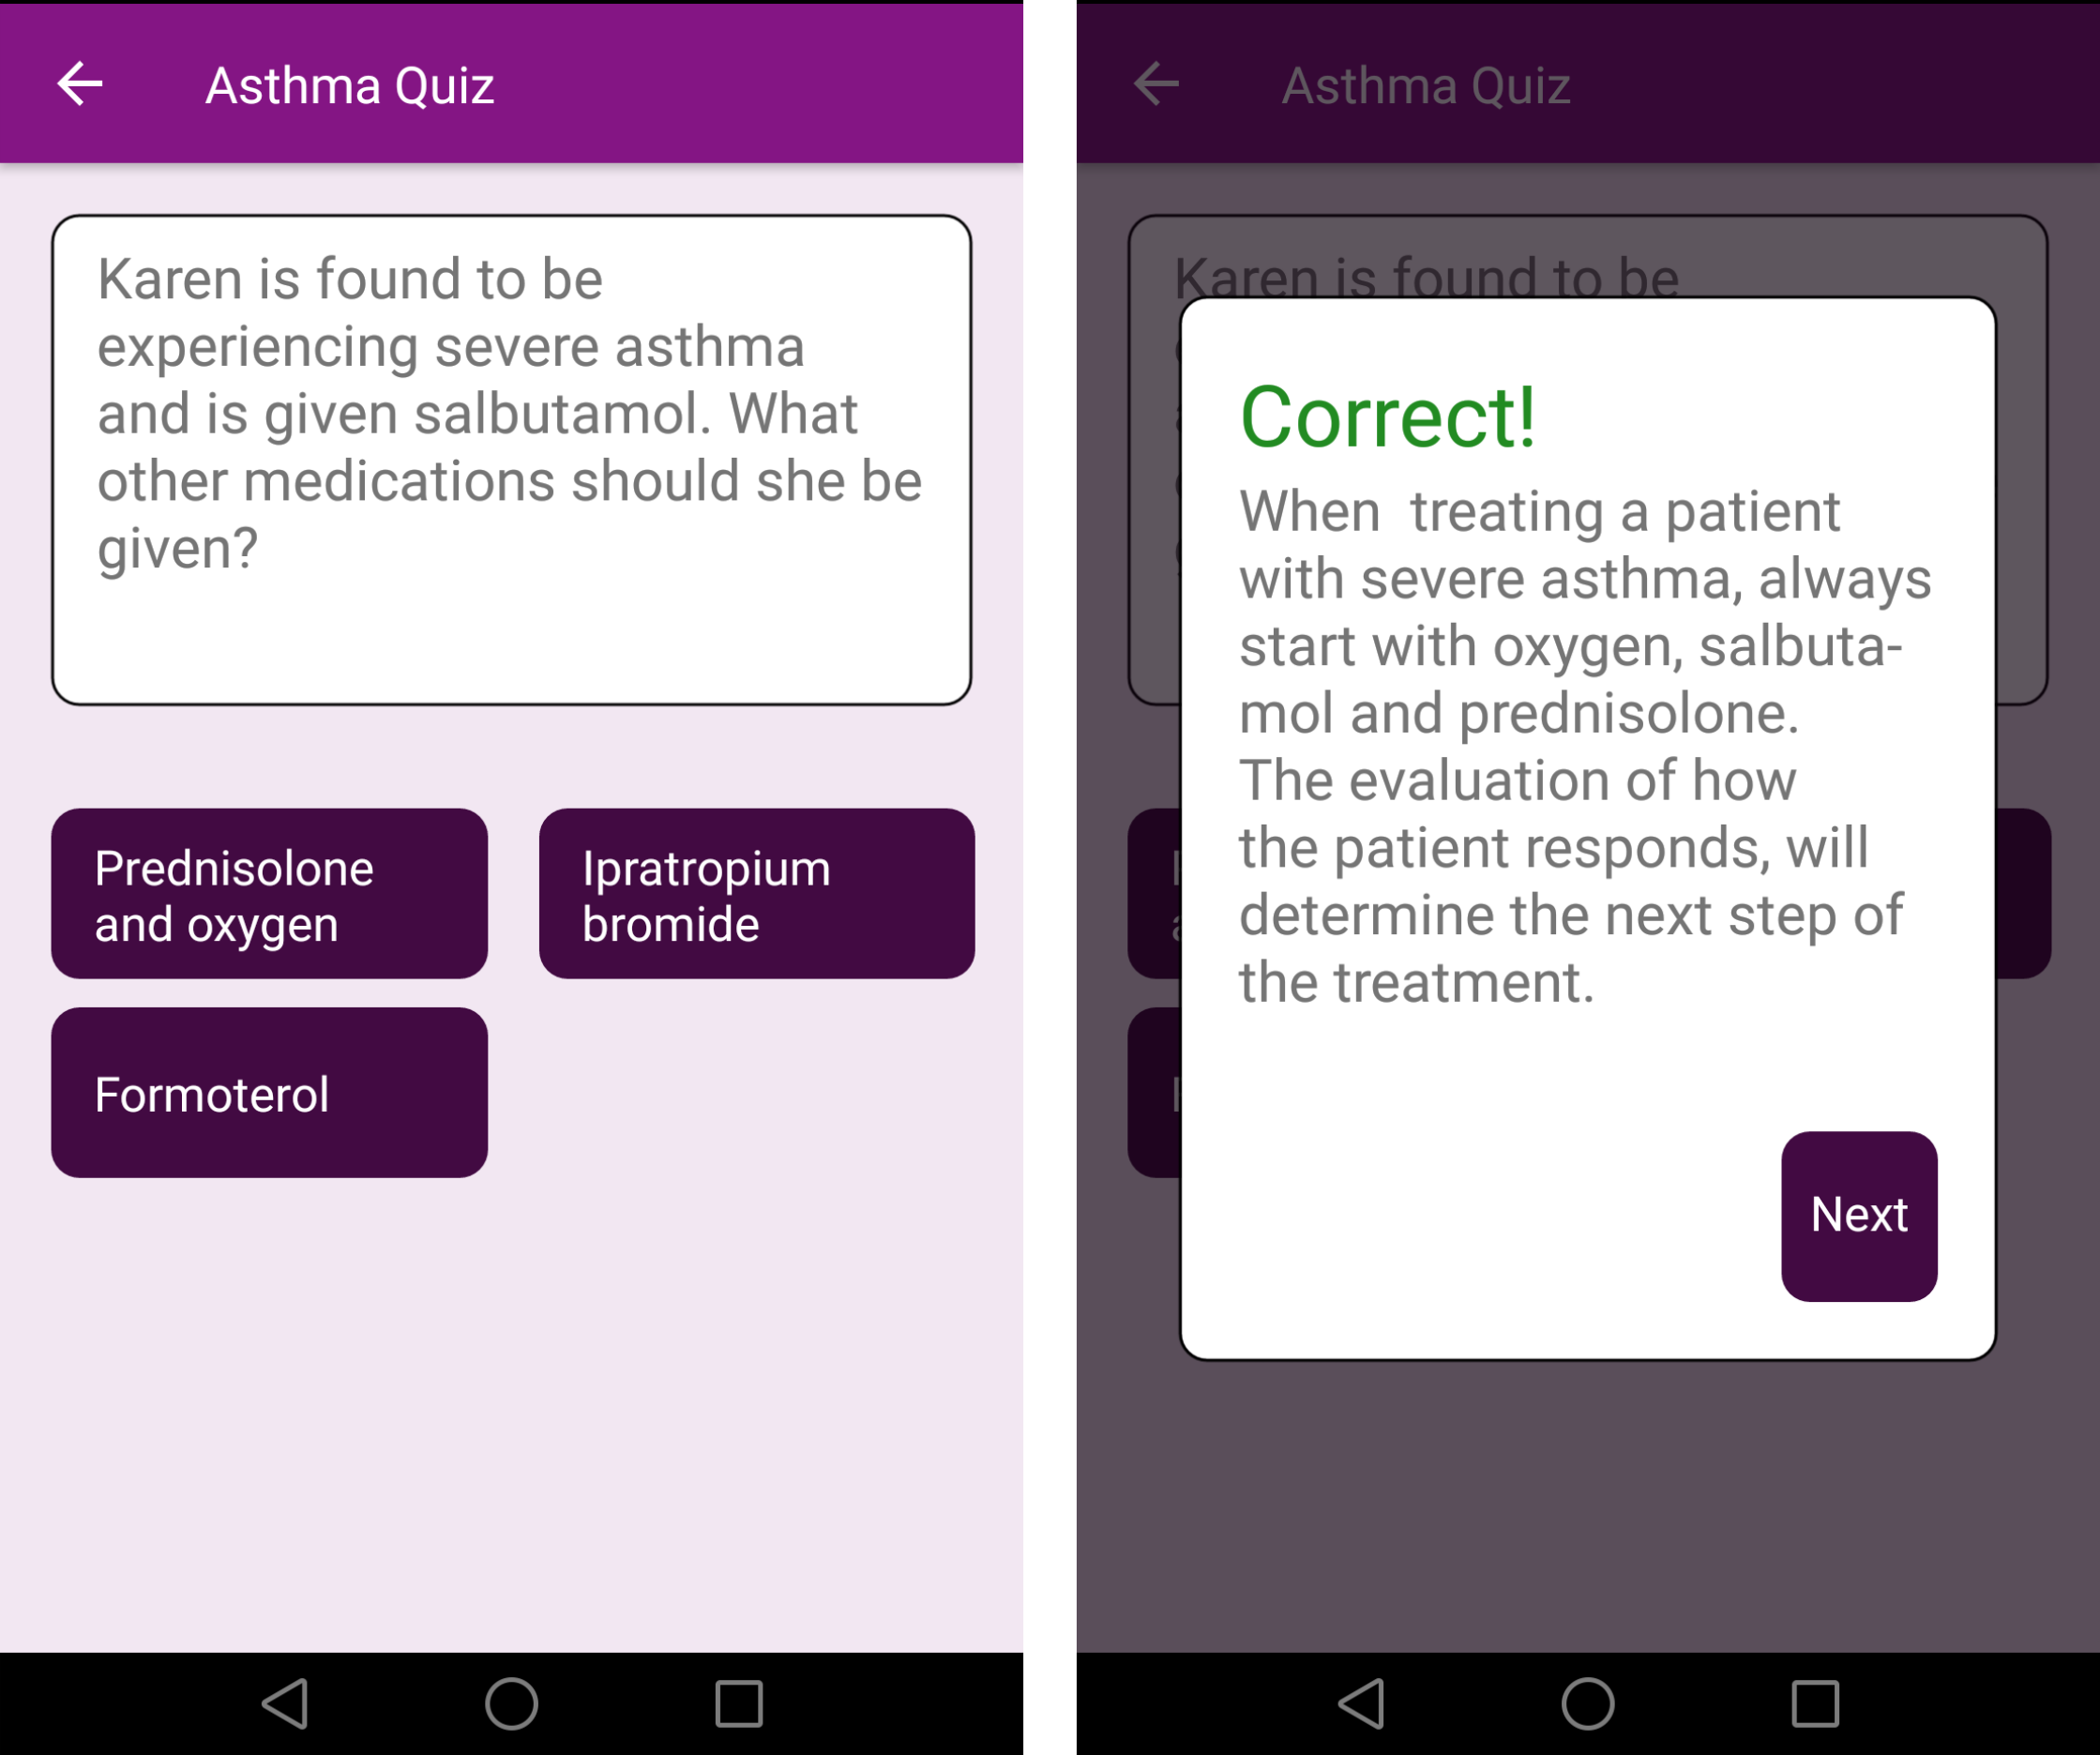
\includegraphics[scale=0.16]{Montage4}
\end{frame}
\begin{frame}{Demonstration}
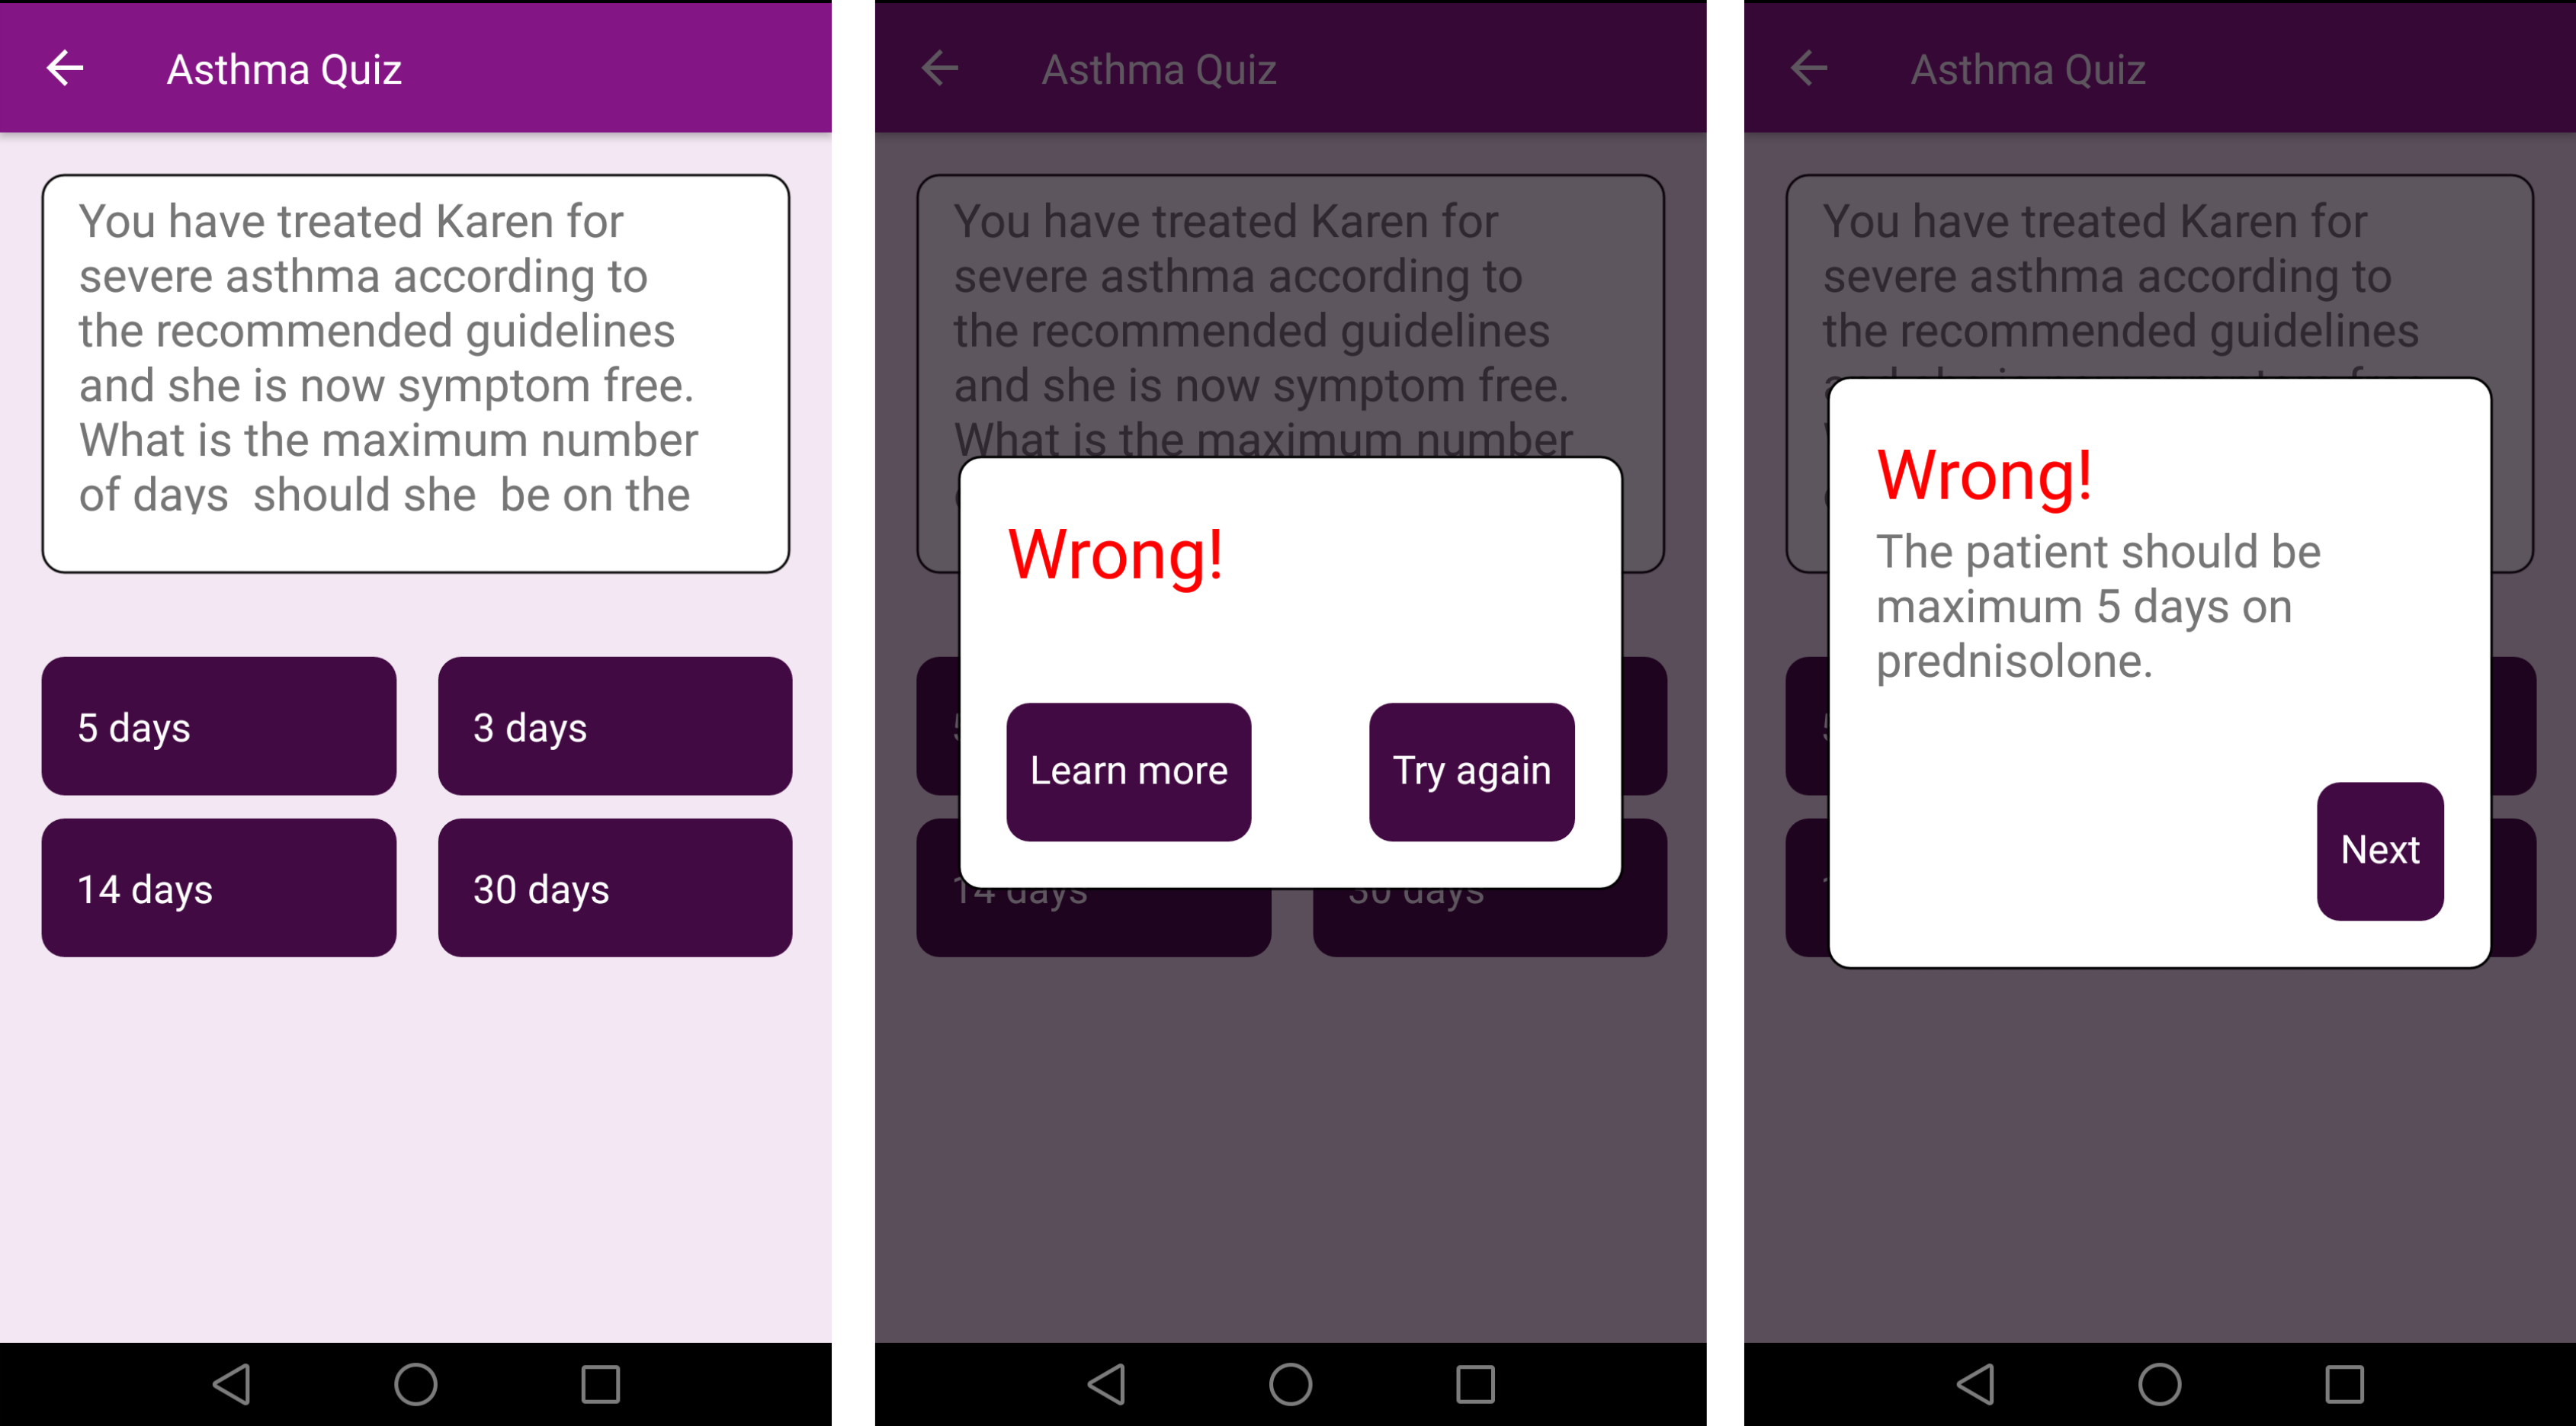
\includegraphics[scale=0.14]{Montage5}
\end{frame}
\begin{frame}{Demonstration}
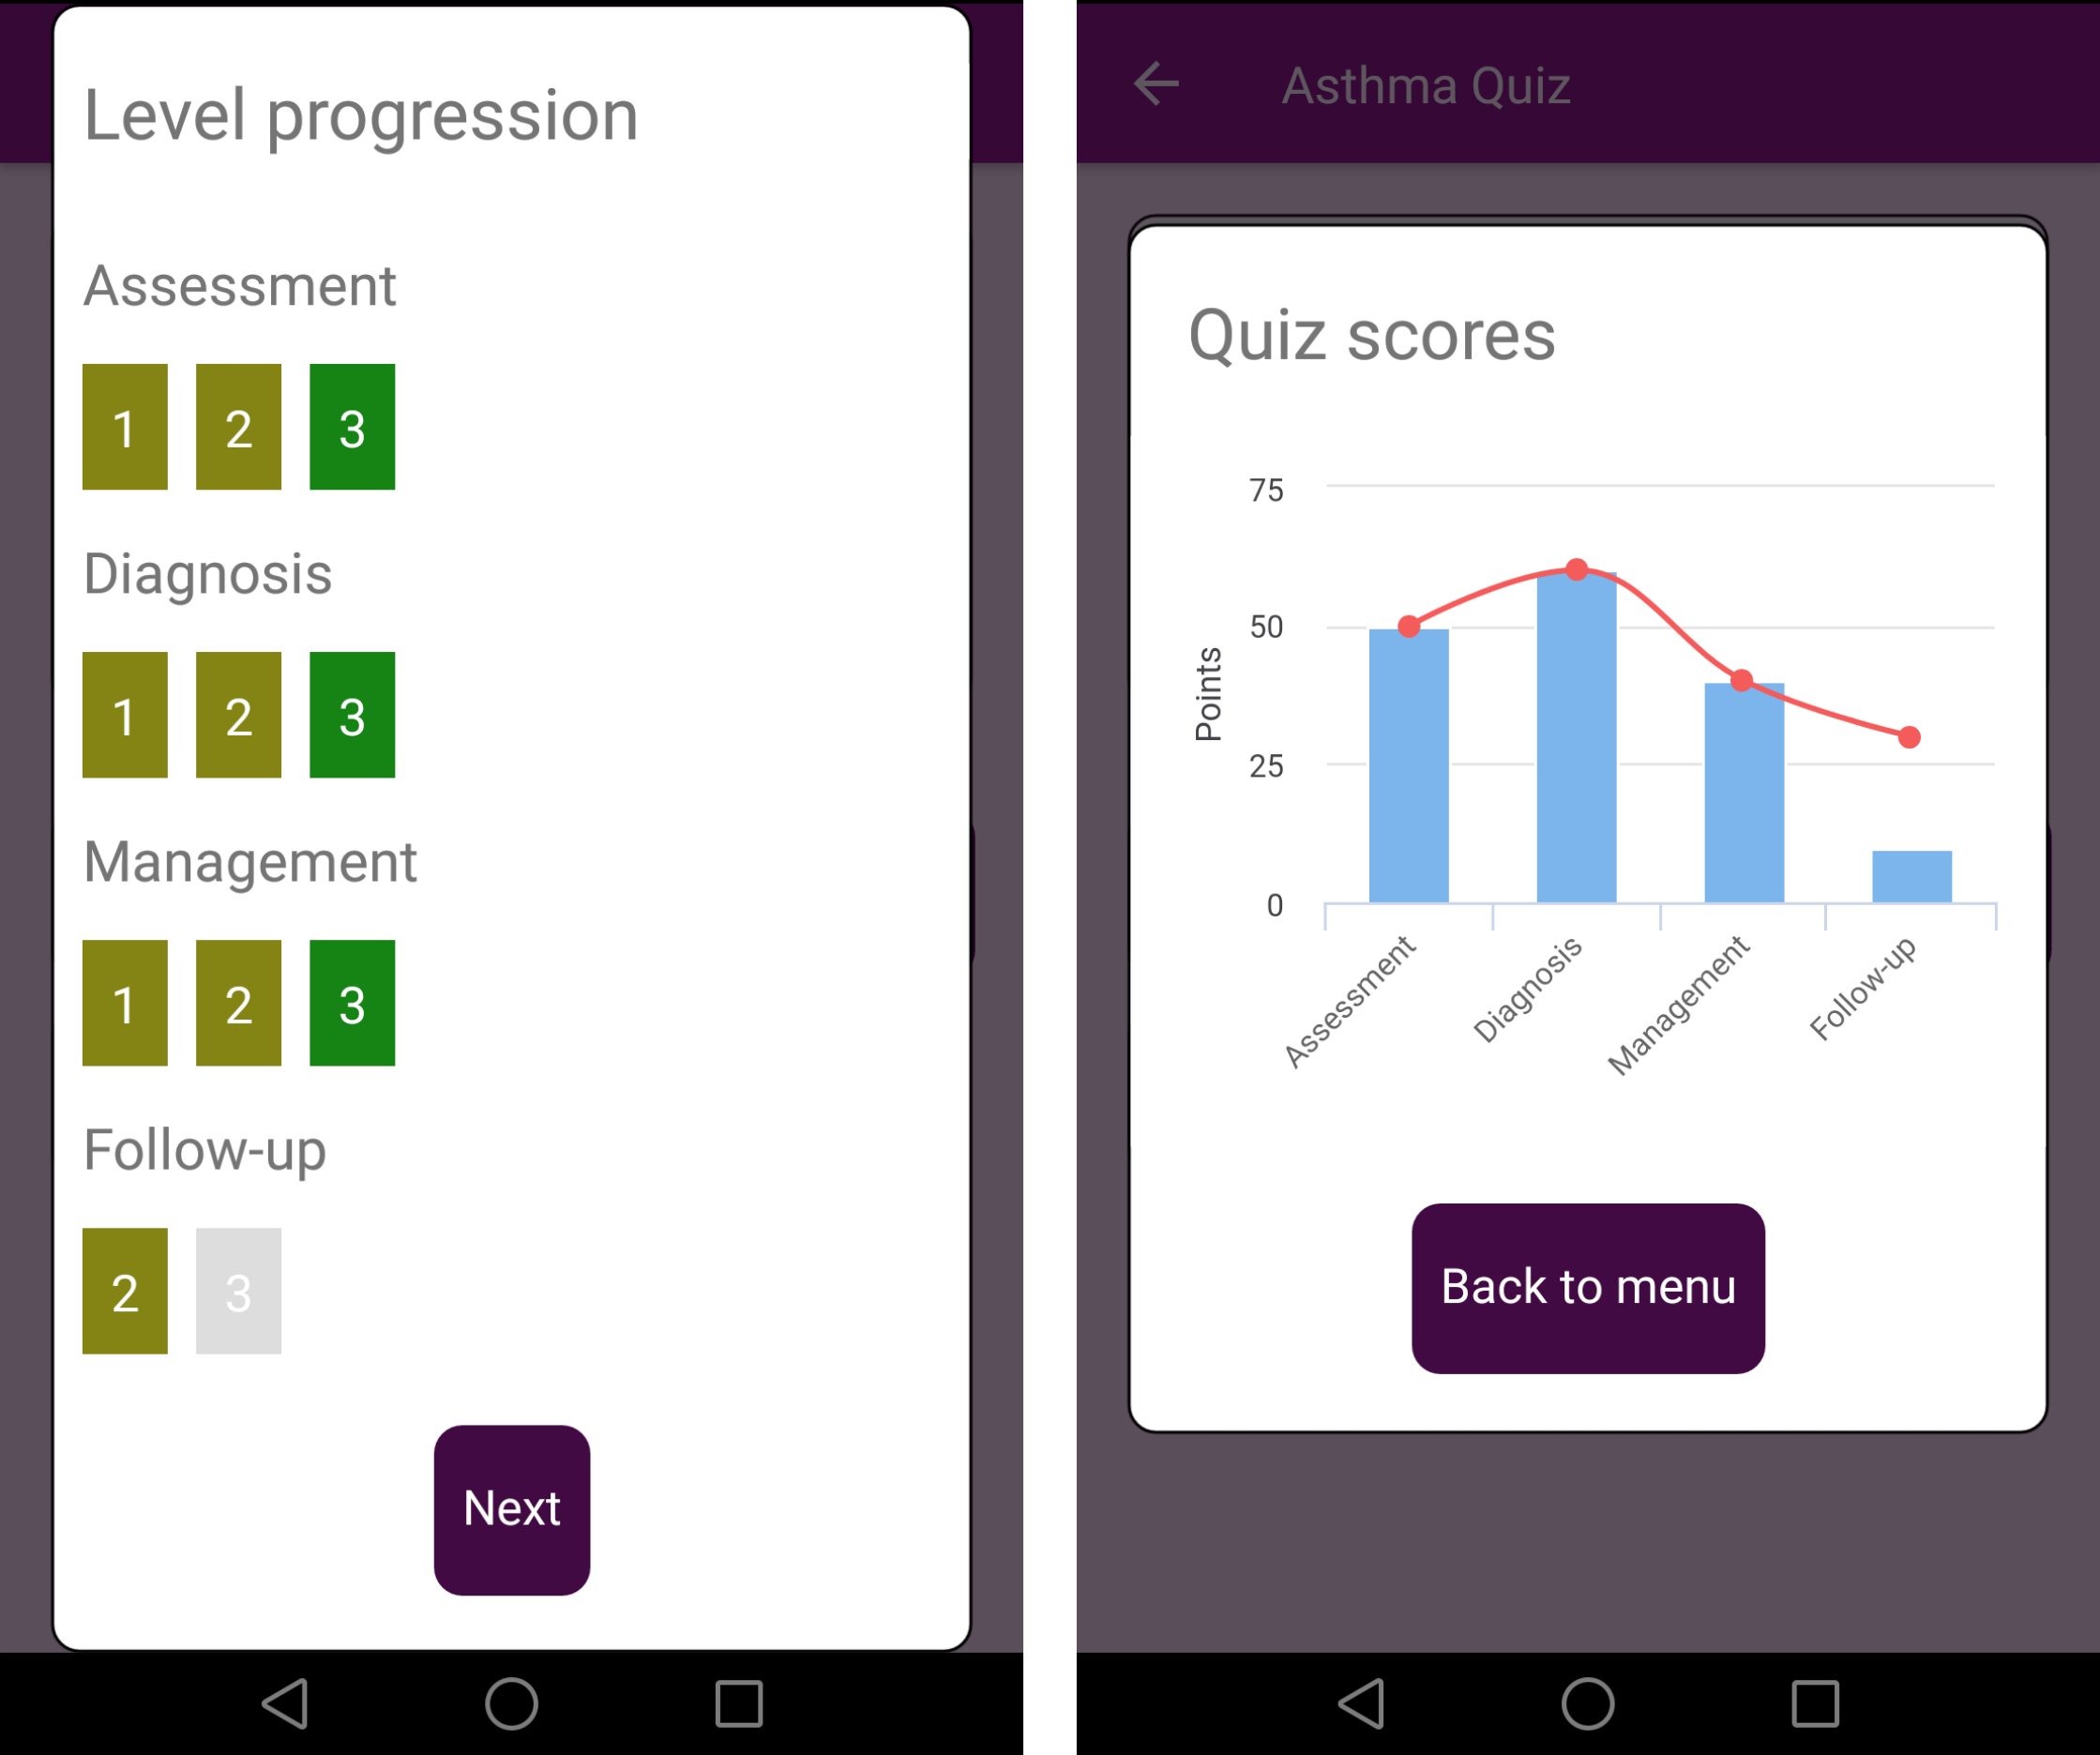
\includegraphics[scale=0.16]{Montage6}
\end{frame}

\begin{frame}{Evaluation}
Planned evaluation
\begin{itemize}
	\item Through user tests, let clinicians or medical students determine the relevance of the artefact.
	\begin{itemize}
		\item Demonstrate how the learning content is adapted to the learners current knowledge level.
	\end{itemize}
	\item Demonstrate that the model can be used to represent other respiratory diseases.
	\item Demonstrate generation of multiple choice questions and answer elements.

\end{itemize}
\end{frame}
\end{document}